% Options for packages loaded elsewhere
\PassOptionsToPackage{unicode}{hyperref}
\PassOptionsToPackage{hyphens}{url}
%
\documentclass[
]{article}
\usepackage{amsmath,amssymb}
\usepackage{iftex}
\ifPDFTeX
  \usepackage[T1]{fontenc}
  \usepackage[utf8]{inputenc}
  \usepackage{textcomp} % provide euro and other symbols
\else % if luatex or xetex
  \usepackage{unicode-math} % this also loads fontspec
  \defaultfontfeatures{Scale=MatchLowercase}
  \defaultfontfeatures[\rmfamily]{Ligatures=TeX,Scale=1}
\fi
\usepackage{lmodern}
\ifPDFTeX\else
  % xetex/luatex font selection
\fi
% Use upquote if available, for straight quotes in verbatim environments
\IfFileExists{upquote.sty}{\usepackage{upquote}}{}
\IfFileExists{microtype.sty}{% use microtype if available
  \usepackage[]{microtype}
  \UseMicrotypeSet[protrusion]{basicmath} % disable protrusion for tt fonts
}{}
\makeatletter
\@ifundefined{KOMAClassName}{% if non-KOMA class
  \IfFileExists{parskip.sty}{%
    \usepackage{parskip}
  }{% else
    \setlength{\parindent}{0pt}
    \setlength{\parskip}{6pt plus 2pt minus 1pt}}
}{% if KOMA class
  \KOMAoptions{parskip=half}}
\makeatother
\usepackage{xcolor}
\usepackage[margin=1in]{geometry}
\usepackage{longtable,booktabs,array}
\usepackage{calc} % for calculating minipage widths
% Correct order of tables after \paragraph or \subparagraph
\usepackage{etoolbox}
\makeatletter
\patchcmd\longtable{\par}{\if@noskipsec\mbox{}\fi\par}{}{}
\makeatother
% Allow footnotes in longtable head/foot
\IfFileExists{footnotehyper.sty}{\usepackage{footnotehyper}}{\usepackage{footnote}}
\makesavenoteenv{longtable}
\usepackage{graphicx}
\makeatletter
\def\maxwidth{\ifdim\Gin@nat@width>\linewidth\linewidth\else\Gin@nat@width\fi}
\def\maxheight{\ifdim\Gin@nat@height>\textheight\textheight\else\Gin@nat@height\fi}
\makeatother
% Scale images if necessary, so that they will not overflow the page
% margins by default, and it is still possible to overwrite the defaults
% using explicit options in \includegraphics[width, height, ...]{}
\setkeys{Gin}{width=\maxwidth,height=\maxheight,keepaspectratio}
% Set default figure placement to htbp
\makeatletter
\def\fps@figure{htbp}
\makeatother
\setlength{\emergencystretch}{3em} % prevent overfull lines
\providecommand{\tightlist}{%
  \setlength{\itemsep}{0pt}\setlength{\parskip}{0pt}}
\setcounter{secnumdepth}{-\maxdimen} % remove section numbering
\ifLuaTeX
  \usepackage{selnolig}  % disable illegal ligatures
\fi
\IfFileExists{bookmark.sty}{\usepackage{bookmark}}{\usepackage{hyperref}}
\IfFileExists{xurl.sty}{\usepackage{xurl}}{} % add URL line breaks if available
\urlstyle{same}
\hypersetup{
  pdftitle={Analytics},
  pdfauthor={Tinotenda Mutsemi (MTSTIN007)},
  hidelinks,
  pdfcreator={LaTeX via pandoc}}

\title{Analytics}
\usepackage{etoolbox}
\makeatletter
\providecommand{\subtitle}[1]{% add subtitle to \maketitle
  \apptocmd{\@title}{\par {\large #1 \par}}{}{}
}
\makeatother
\subtitle{Assignment 1}
\author{Tinotenda Mutsemi (MTSTIN007)}
\date{2024-03-05}

\begin{document}
\maketitle

\hypertarget{question-1}{%
\section{Question 1}\label{question-1}}

\hypertarget{question-1a}{%
\subsection{Question 1a}\label{question-1a}}

We split the data into training and test sets using an 80/20 split.

We fit a homegrown tree by setting the minimum size of the terminal
nodes to 2 and the minimum deviance to 0.

This tree is overfitted, and we see that loacation features and count
result in the most misclassification error reduction.

\begin{figure}
\centering
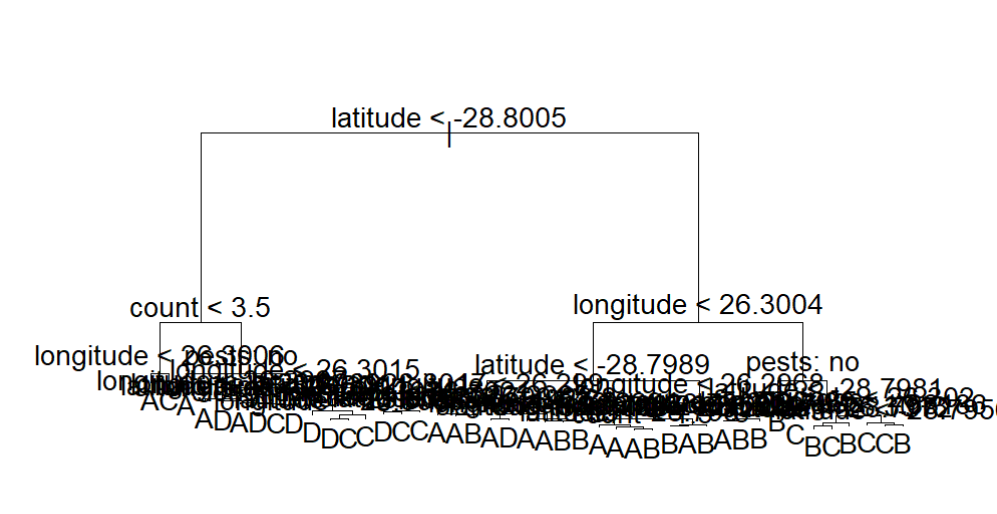
\includegraphics[width=4.51042in,height=\textheight]{big_tree_mealies.png}
\caption{Overfitted Homogenous Mealies Tree}
\end{figure}

We then test the perfomance with the 20\% we splitted from the data.
Below is the confusion matrix of the test showing a misclassification
rate of 8\%.

\begin{longtable}[]{@{}lllll@{}}
\toprule\noalign{}
& A Predicted & B Predicted & C Predicted & D Predicted \\
\midrule\noalign{}
\endhead
\bottomrule\noalign{}
\endlastfoot
A Actual & 40 & 3 & 0 & 1 \\
B Actual & 2 & 70 & 1 & 0 \\
C Actual & 0 & 1 & 31 & 5 \\
D Actual & 4 & 0 & 3 & 89 \\
\end{longtable}

\hypertarget{question-1b}{%
\subsection{Question 1b}\label{question-1b}}

We use cross validation to prune the tree. We use 10 fold cross
validation and the misclassification error as the cost function. We plot
the cross validation error against the number of terminal nodes and the
penality alpha.

\begin{figure}
\centering
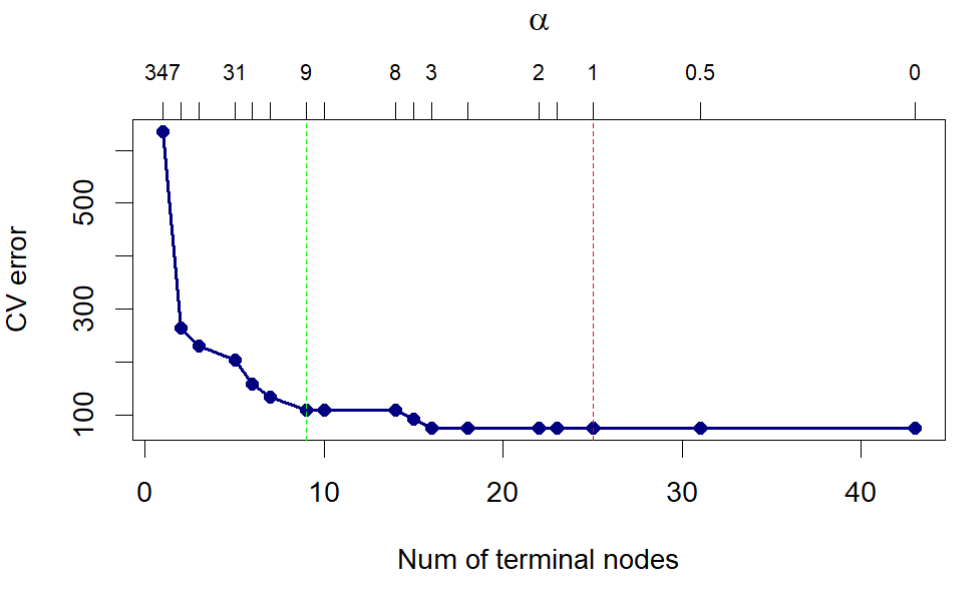
\includegraphics[width=4.32292in,height=\textheight]{cv_error_num_nones_mealies.png}
\caption{CV error for each tree size}
\end{figure}

We see the tree with the minimum cross validation error (red) line has
over 20 nodes. We choose the tree with 9 nodes (green line) because it
has good interpretability at a low error rate, compared to the lost of
interpretability we get from the minimal error tree. The pruned tree has
a misclassification rate of 13.2\% and the confusion matrix is shown
below.

These results are worse than from an overfitted tree. This tree has a
higher cross validation error as shown by the fig above with CV error
size for each tree. Therefore this is expected. We however gain
interpretability at the cost of a sightly higher missclassification
rate.

\begin{longtable}[]{@{}lllll@{}}
\toprule\noalign{}
& A Predicted & B Predicted & C Predicted & D Predicted \\
\midrule\noalign{}
\endhead
\bottomrule\noalign{}
\endlastfoot
A Actual & 30 & 10 & 1 & 4 \\
B Actual & 1 & 71 & 1 & 0 \\
C Actual & 0 & 3 & 22 & 12 \\
D Actual & 0 & 2 & 0 & 94 \\
\end{longtable}

\hypertarget{question-1c}{%
\subsection{Question 1c}\label{question-1c}}

We plot the location of the mealies on a scatter plot with the quality
of the mealies represented by the color of the points. Tree methods
partion the feature space othogonally and therefore we rotate the
feature space to see if we can get a better partitioning of the feature
space.

\begin{figure}
\centering
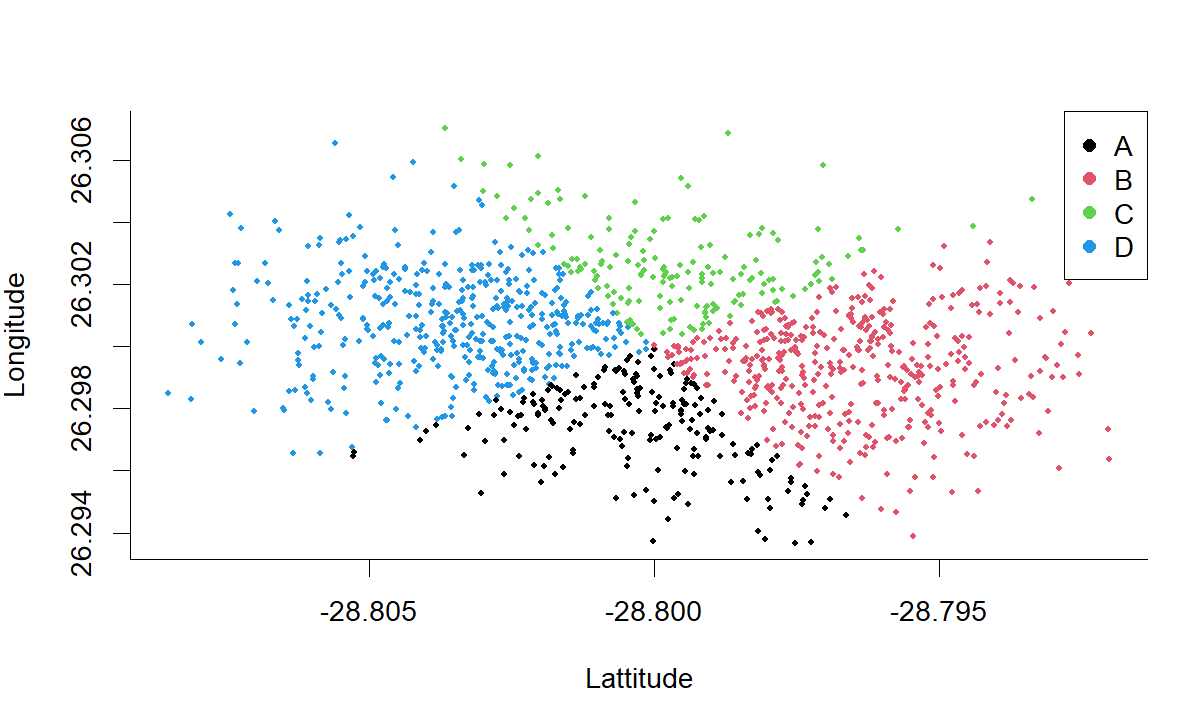
\includegraphics[width=4.84375in,height=\textheight]{feature_space_mealies.png}
\caption{Mealies feature space}
\end{figure}

Now we apply 10 fold cross validation to the rotated data. We rotate the
feature space over thetas. We then plot the misclassification error
against the rotation angle. We see that the misclassification error is
lowest at 0.97

\begin{figure}
\centering
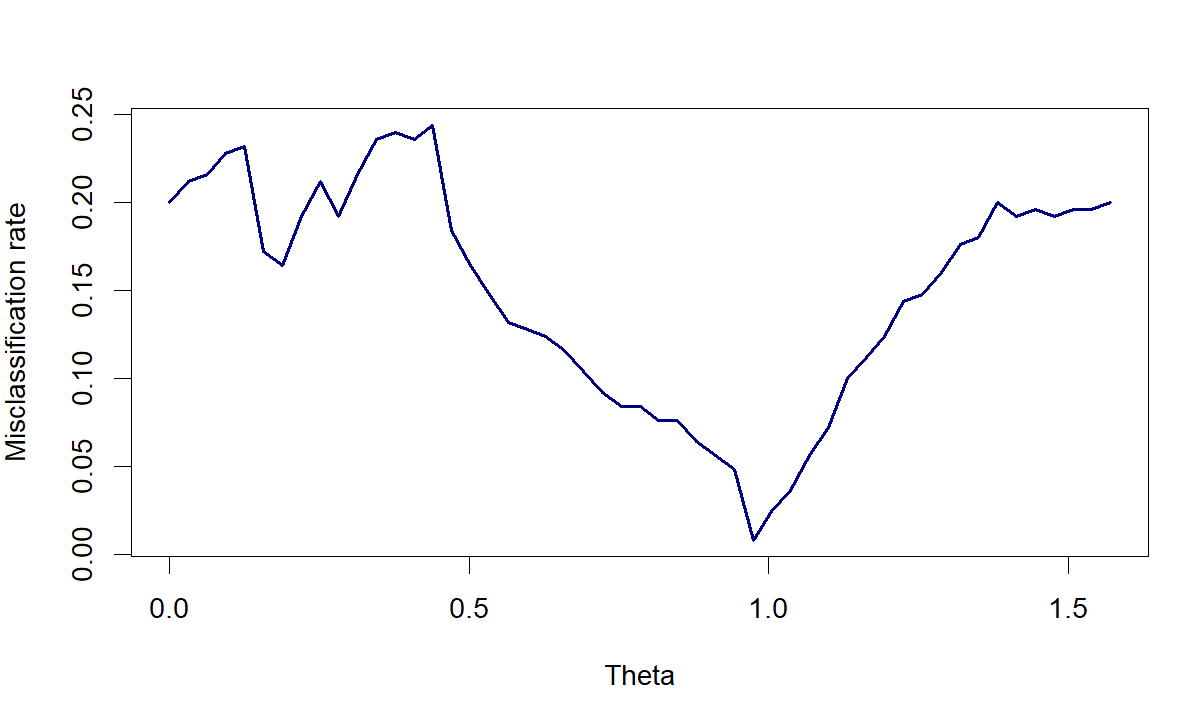
\includegraphics[width=4.41667in,height=\textheight]{misclass_theta_mealies.png}
\caption{Misclassification rates for theta}
\end{figure}

The misclassification rate is 0.4\%. This is expected because the tree
method partions the feature space orthogonally and therefore rotating
the feature space will find lower misclassification rates.

Below is the confusion matrix for the rotated feature space. This tree
perform very well even on unseen data.

\begin{longtable}[]{@{}lllll@{}}
\toprule\noalign{}
& A Predicted & B Predicted & C Predicted & D Predicted \\
\midrule\noalign{}
\endhead
\bottomrule\noalign{}
\endlastfoot
A Actual & 44 & 0 & 0 & 0 \\
B Actual & 0 & 73 & 0 & 1 \\
C Actual & 0 & 0 & 37 & 0 \\
D Actual & 0 & 0 & 0 & 95 \\
\end{longtable}

\hypertarget{question-2}{%
\section{Question 2}\label{question-2}}

We do some exploratory analysis to see the variables correlation.

Below is the scatter plot of First Inn Score and Bowl2 Strength. We can
see that there is a positive correlation between the two variables.

We remove the match id from the regression, standardize the data and use
dummy variables for the categorical variables.

We also remove defending team and chasing team from the regression. As
they are not consistent across seasons.

\begin{figure}
\centering
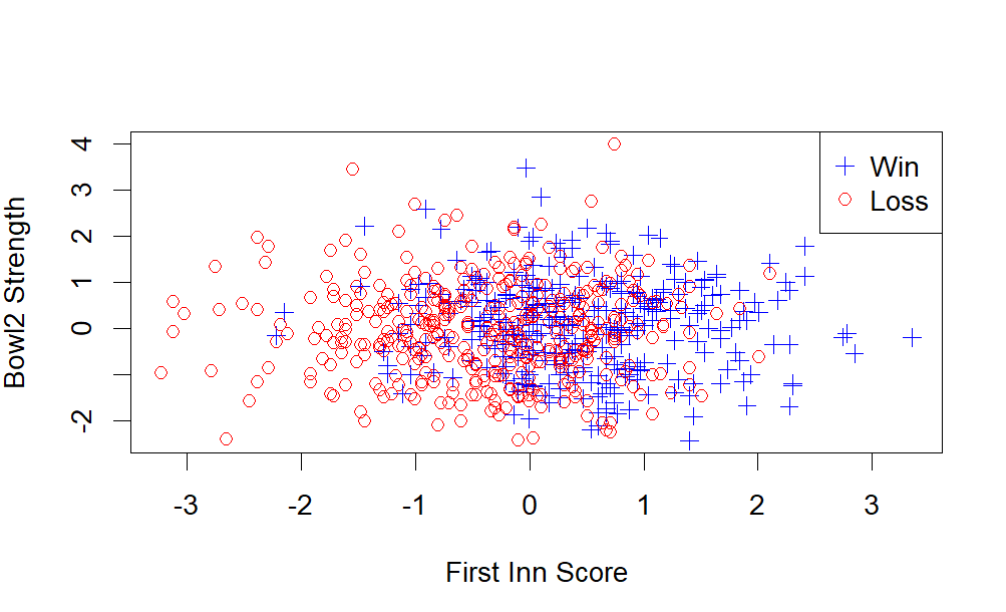
\includegraphics[width=4.63542in,height=\textheight]{scatter_first_innsscore.png}
\caption{First Inn Score vs the team Bowling in the second round}
\end{figure}

\hypertarget{question-2a}{%
\subsection{Question 2a}\label{question-2a}}

We fit check the model after feature selection and standardization.

Now we fit an elastic net model to the data. We use cross validation to
select the best alpha and lambda. We sequence alpha from 0 to 1 and use
10 fold cross validation to select the best lambda for each alpha.

The plot below shows the misclassificatioin rates for each alpha. The
best alpha is 0.3

\begin{figure}
\centering
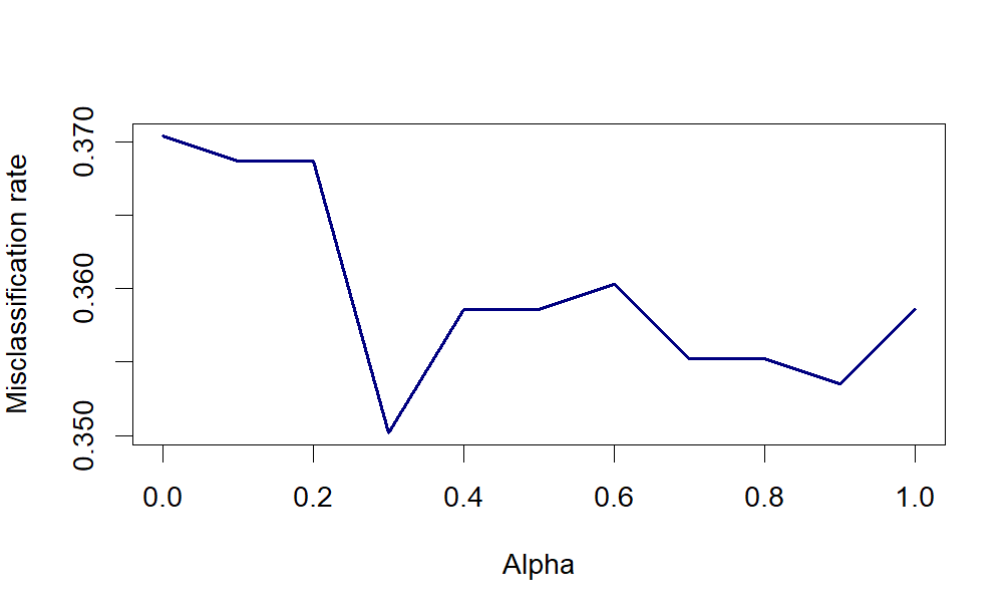
\includegraphics{misclass_rate_ipl.png}
\caption{Misclassification Rates for each Alpha at the best Lambda}
\end{figure}

We fit the elastic net model with alpha = 0.3 and plot the coefficients.
The best lambda is 0.28.

We see that at these hyperparameter we only have 1 feature in the model.

\begin{figure}
\centering
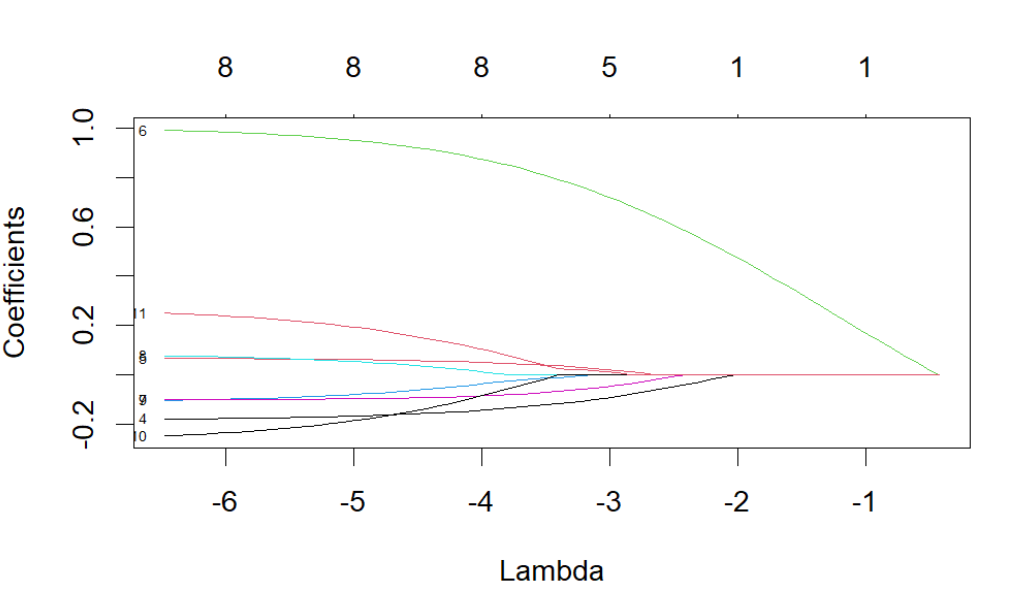
\includegraphics{coef_ipl.png}
\caption{Coefficients at lambda 0.28 is First Inn Score only}
\end{figure}

First Inn Score with a coefficient of 0.25. This means that a unit
increase in the first innings score increases the log odds of winning by
0.25.

Below is the confusion matrix from testing the model.

\begin{longtable}[]{@{}lll@{}}
\caption{Confusion Matrix}\tabularnewline
\toprule\noalign{}
& Loss Predicted & Win Predicted \\
\midrule\noalign{}
\endfirsthead
\toprule\noalign{}
& Loss Predicted & Win Predicted \\
\midrule\noalign{}
\endhead
\bottomrule\noalign{}
\endlastfoot
Loss Actual & 80 & 10 \\
Win Actual & 40 & 19 \\
\end{longtable}

The F score is 0.43 showing that the model is not good because the F1
score is less than 0.5.

\hypertarget{question-2b}{%
\subsection{Question 2b}\label{question-2b}}

\hypertarget{question-3}{%
\section{Question 3}\label{question-3}}

\hypertarget{question-3a}{%
\subsection{Question 3a}\label{question-3a}}

We do some exploratory analysis to see the variables correlation.

\begin{figure}
\centering
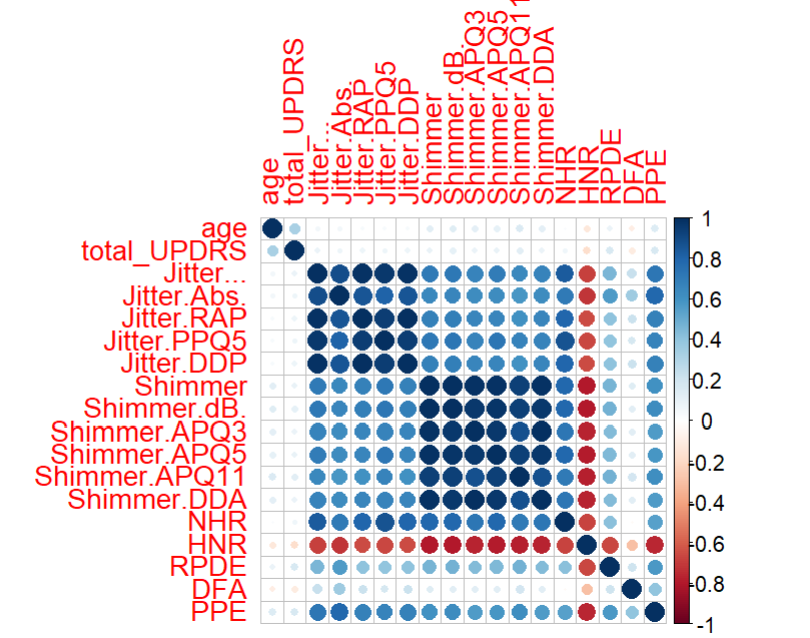
\includegraphics[width=3.76042in,height=\textheight]{corr_parkinsons.png}
\caption{Variable correlations for Parkinsons data set}
\end{figure}

The table below shows the covariance, p value, and the correlation
coefficient for the variables in the Parkinsons data set.

\hypertarget{question-3a-i}{%
\subsubsection{Question 3a i}\label{question-3a-i}}

We fit an elastic net with alpha = 1 for lasso regularization.

Our final model (min lambda.1se) has test MSE of 95, and variables age,
sex, DFA with high significance.

The plot shows lambda and MSE for the elastic net model.

\begin{figure}
\centering
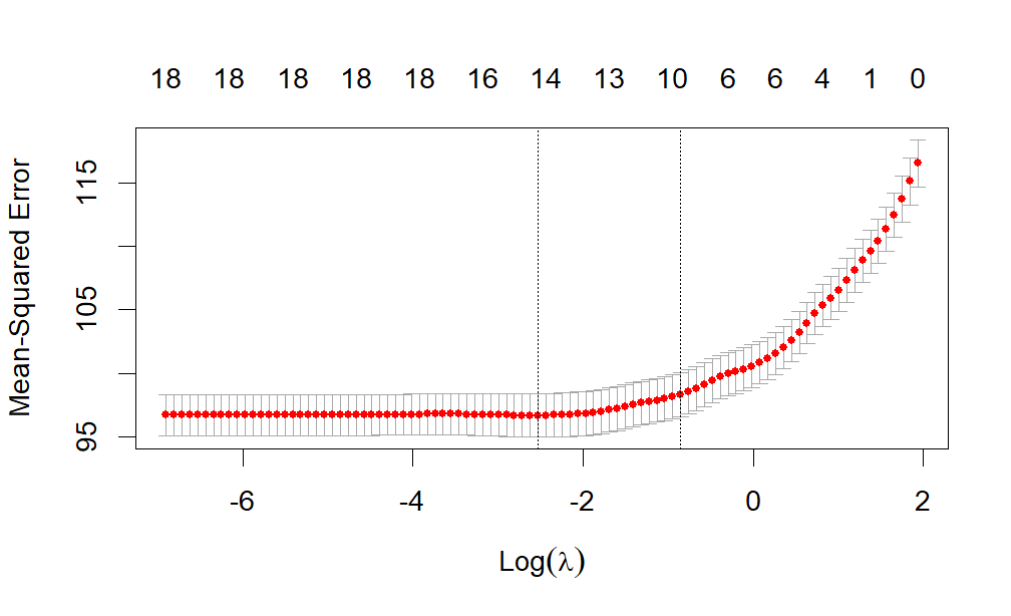
\includegraphics[width=4.85417in,height=\textheight]{mse_elastic_net.png}
\caption{MSE Elastic net over lambda}
\end{figure}

\hypertarget{question-3a-ii}{%
\subsubsection{Question 3a ii}\label{question-3a-ii}}

We range k from 1 to 15 and set up the control for model training using
10-fold cross-validation, repeated 10 times to provide a robust estimate
of model performance.

The choose k = 4 because it has the lowest RMSE.

\begin{figure}
\centering
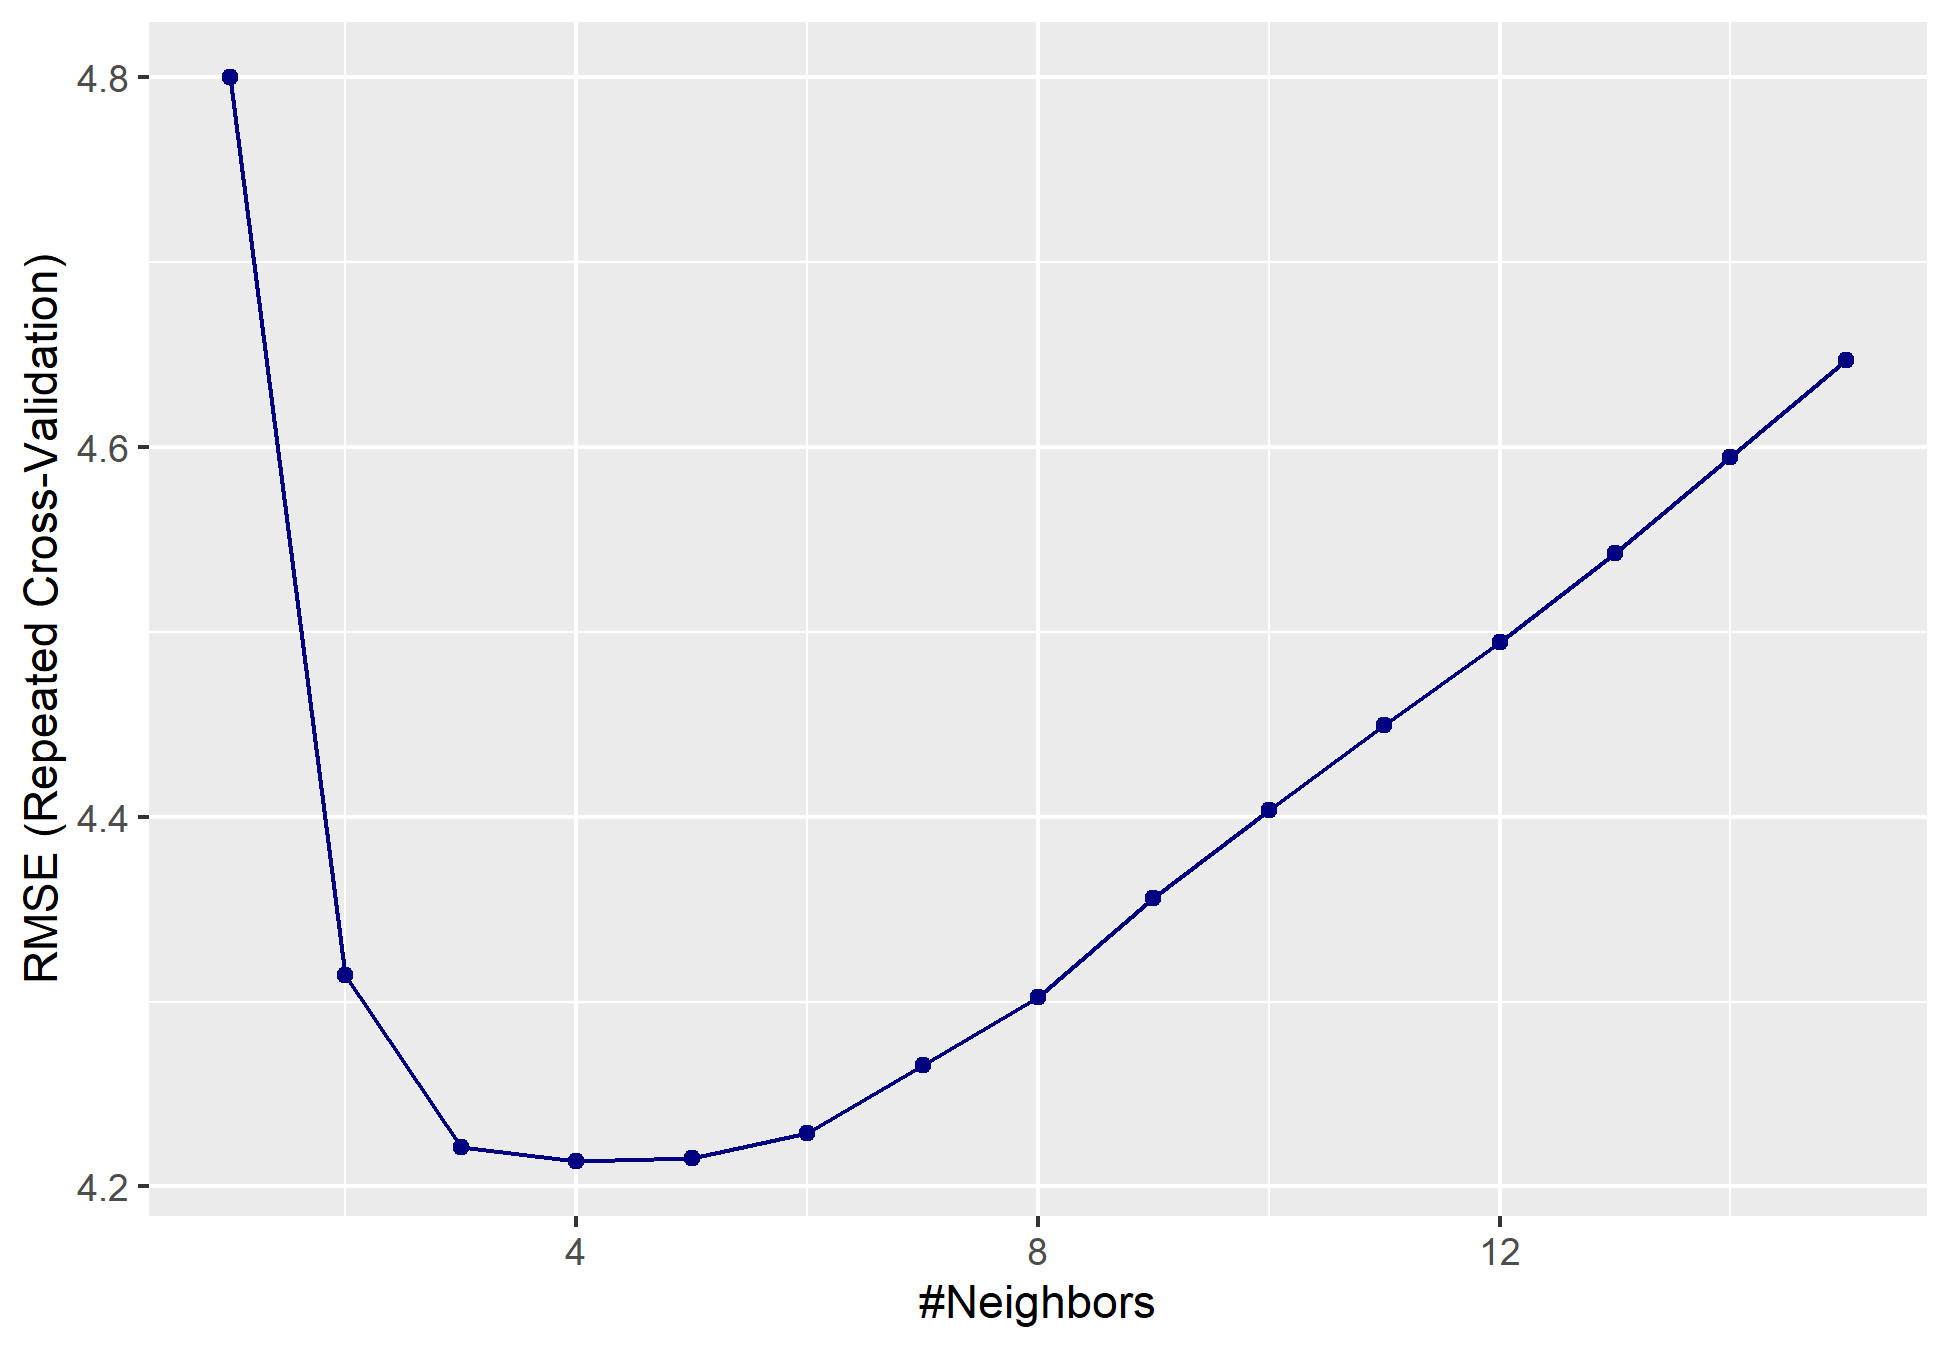
\includegraphics[width=4.875in,height=\textheight]{rmse_knn.png}
\caption{RMSE of KNN from k = 1 to 15}
\end{figure}

\hypertarget{question-3a-iii}{%
\subsubsection{Question 3a iii}\label{question-3a-iii}}

Now we train a random forest model using ranger and caret. Number of
variables randomly sampled as candidates at each split in the decision
tree is varied from 2 to 20, and the minimum node size is 1, 5, 10, 15,
20. We use 10-fold cross-validation, repeated 10 times to provide a
robust estimate of model performance.

The est MSE of 8.75.

\begin{figure}
\centering
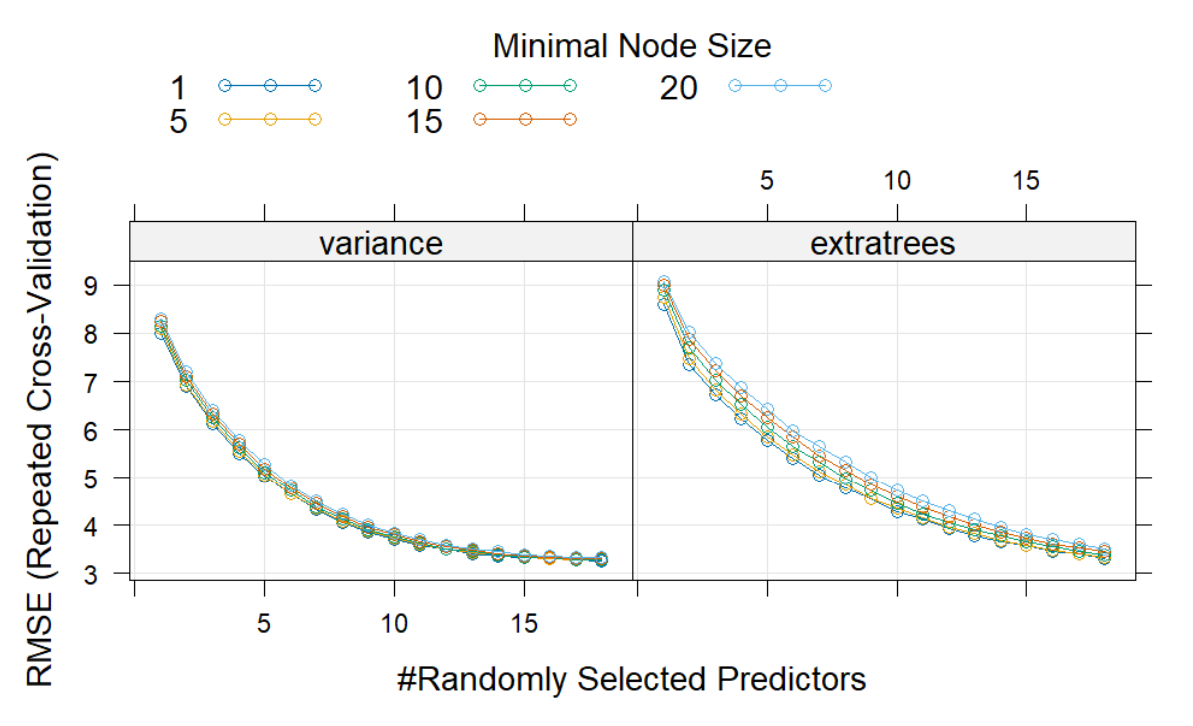
\includegraphics[width=6.22917in,height=\textheight]{rmse_random_forest.png}
\caption{Random forests grid RMSE}
\end{figure}

\hypertarget{question-3a-iv}{%
\subsubsection{Question 3a iv}\label{question-3a-iv}}

We now fit the model using the xgboost algorithm. We search for the best
hyperparameters using a grid search set to 100 boosting rounds and
10-fold cross validation repeated 10 times. We then fit the model using
the best hyperparameters and predict the test data.

Below is the variable importance plot for the xgboost model. We notice
that after the 8th variable the importance is 0. The most important
features are age, DFA and sex.

\begin{figure}
\centering
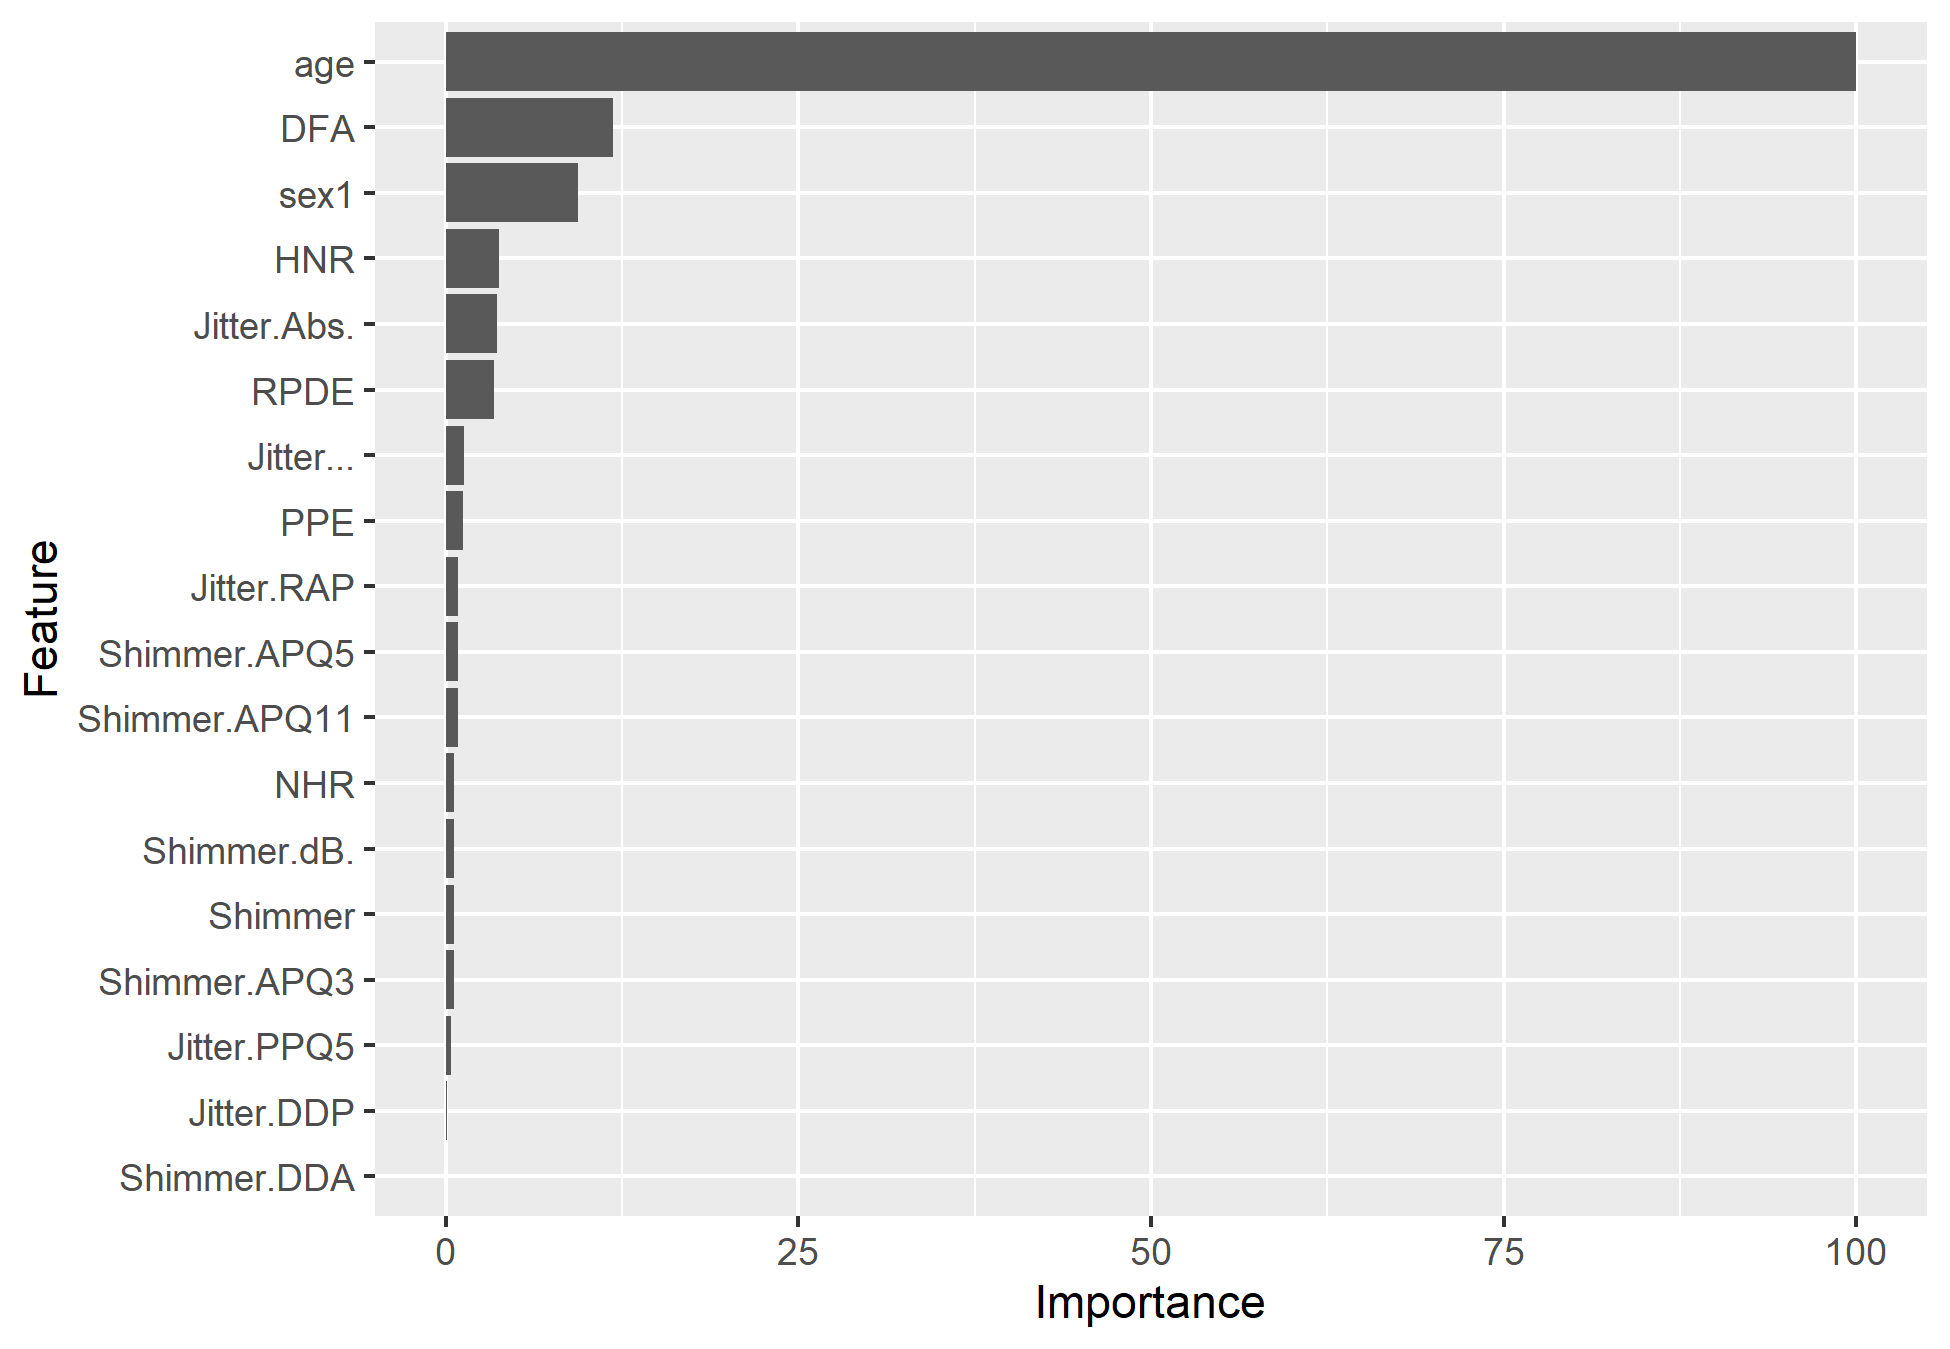
\includegraphics[width=4.07292in,height=\textheight]{varimpo_xgboost.png}
\caption{XGBoost Variable Importance}
\end{figure}

\hypertarget{question-3b}{%
\subsection{Question 3b}\label{question-3b}}

The table below shows the MSE of the 4 different models. XGBoost
produces the least MSE, and we shall choose it as the best model and use
it to test the data performance with Q3testing.csv.

\begin{longtable}[]{@{}ll@{}}
\toprule\noalign{}
Model & MSE \\
\midrule\noalign{}
\endhead
\bottomrule\noalign{}
\endlastfoot
Elastic net & 95.59 \\
KNN & 14.90 \\
Random forest & 19.70 \\
XGBoost & 9.00 \\
\end{longtable}

Below is the plot showing the RMSE of the XGBoost model. The selected
model has a depth of 8. There is a low RMSE however its weakness is lack
of interpretability. For lesser tree depths, where we have good
interpretability, the RMSE has not yet converged.

\begin{figure}
\centering
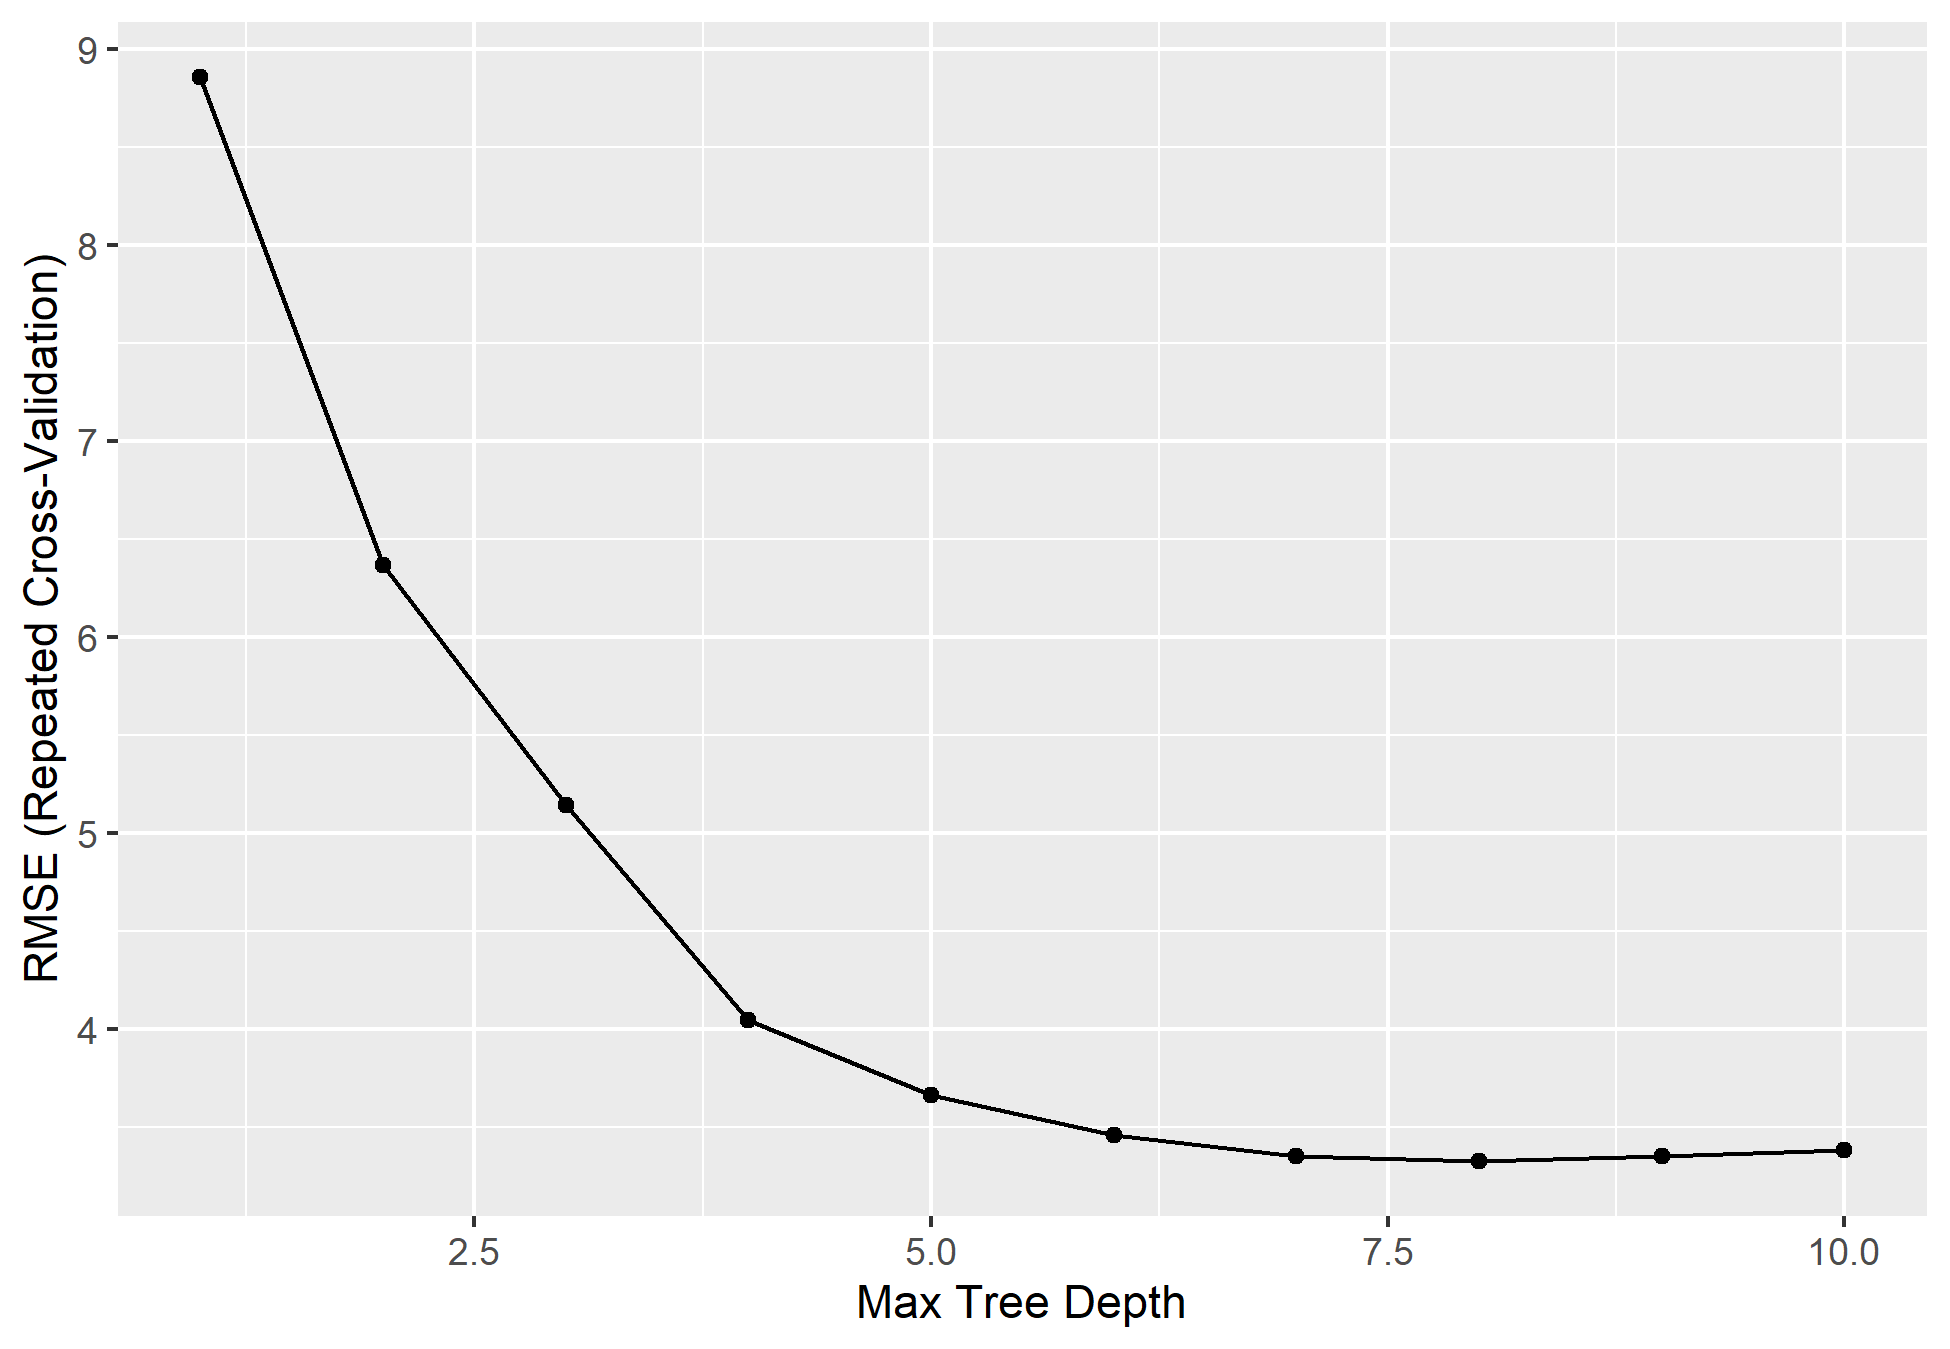
\includegraphics[width=4.36458in,height=\textheight]{rmse_xgboost.png}
\caption{RMSE vs Maximum tree depth.}
\end{figure}

\hypertarget{question-3c}{%
\subsection{Question 3c}\label{question-3c}}

The predictions for Q3testing are in MTSTIN007.csv.

\end{document}
